\documentclass{article}
\usepackage{graphicx}
\usepackage[top=0.8in, bottom=0.8in, left=0.8in, right=0.8in]{geometry}
\usepackage{float}

\title{Parallel Implementation of LU decomposition}
\author{Adil Ansari}

\begin{document}
\maketitle

\section{Basics}
\begin{itemize}
\item Root directory contains three sub-directories namely 'Sequential', 'OpenMP' and 'MPI'.
\item Each subdirectory has source code in the form of \textbf{ '*.c'} file.
\item Matrix is generated in a manner that it decomposes into a L and U containing only 1s and 0s.
\item To submit jobs for various configurations run \textbf{'./submit.sh'} on terminal. This will automatically submit all the jobs in the subdirectory to the \textbf{general-compute} queue of the ccr cluster.
\item Outputs are generated in the /textbf{output.txt} file. \textit{Sample outputs are included}.
\item In the corresponding subdirectory run \textbf{./plot.sh} on the linux terminal to generate a graphical visualization of the output. \textit{gnuplot is required to generate graph}.
\item Graphs are generated as \textbf{'Plot.pdf'}. \textit{Please wait for the job run to finish and outputs to accumulate}.
\end{itemize}

\section{Sequential Implementation}
\begin{itemize}
\item Gaussian elimination algorithm was implemented that sequentially decomposes the square matrix. 
\item Algorithm was evaluated on input matrix size of 1000, 5000, 10000, 20000. 
\item Time taken to decompose the matrix grew exponentially with the increase in size.
\item Since, this was a sequential implementation increase in compute nodes won't do anything.
\item Since I was using Gaussian elimination that computes L and U matrices separately, I ran \textbf{out of memory} when matrix size of 50,000 was tried. This implementation makes two copies of the matrix of same size as input.
\end{itemize}

\begin{figure}[H]
\begin{center}
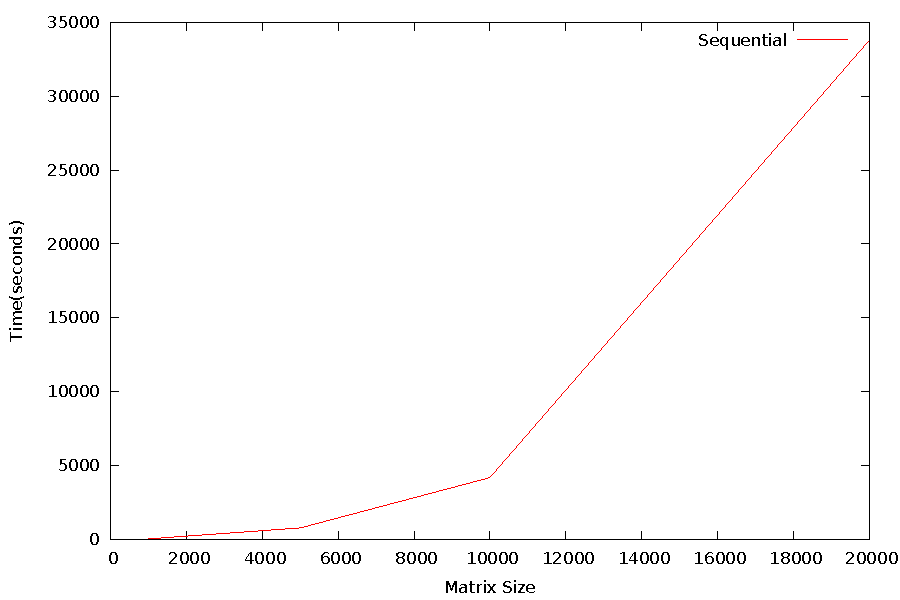
\includegraphics[height=3in,width=5in]{Sequential/Plot.pdf}
\caption{Sequential Decomposition Algorithm}
\end{center}
\end{figure}

\section{OpenMP Implementation}
\begin{itemize}
\item Gaussian elimination algorithm was implemented that uses the block wise decomposition in parallel.
\item The \textbf{for} loops are parallelized in a manner that blocks of matrices are decomposed by dividing the work among parallel threads.
\item Algorithm was evaluated for input matrix of sizes 1000, 5000, 10000, 20000 with a combination of 2, 4, 8, 16, 32 threads executing in parallel.
\item On a fixed workload the decompostion was faster when more threads are executing in parallel. The execution was comparatively faster on larger workload due to the fact, parallelism was more effective.

\begin{figure}[H]
\begin{center}
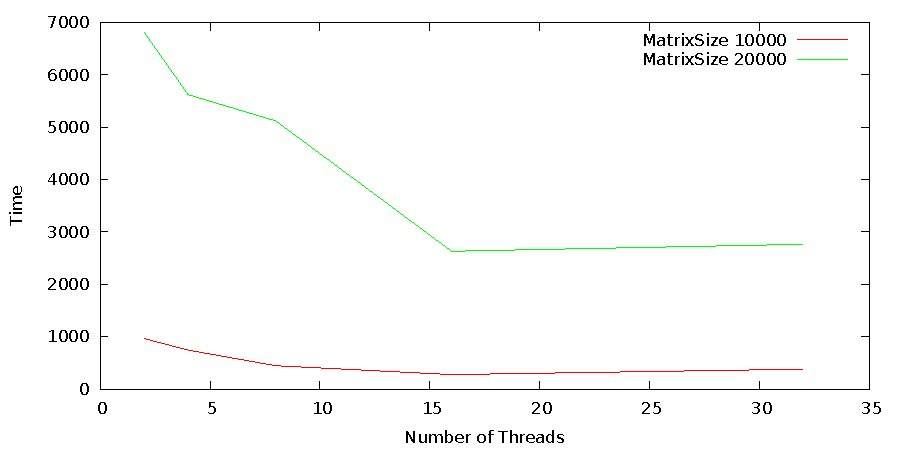
\includegraphics[height=3in,width=5in]{Graphs/omp_core_time.pdf}
\caption{OpenMP Performance for fixed Matrix Size}
\end{center}
\end{figure}

\item For a fixed number of cores the time increased exponentially with increase in matrix size.

\begin{figure}[H]
\begin{center}
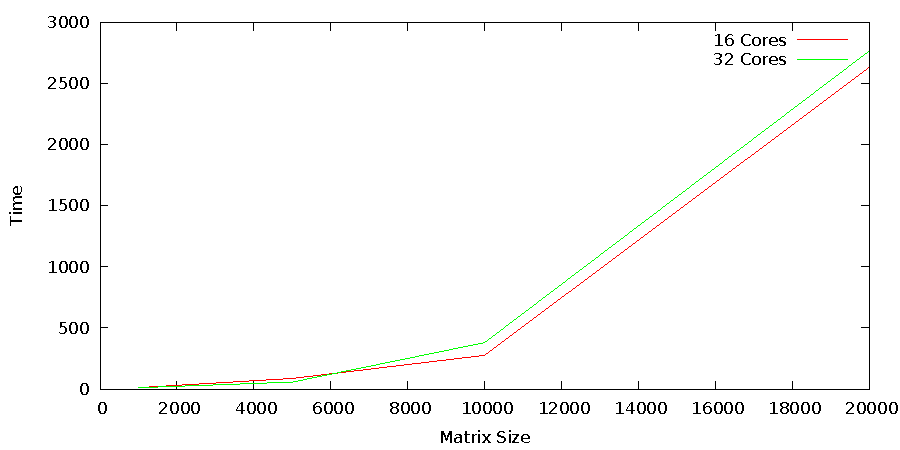
\includegraphics[height=3in,width=5in]{Graphs/omp_siz_time.pdf}
\caption{OpenMP Performance for fixed Number of Cores}
\end{center}
\end{figure}


\item The parallelism was ineffective on relatively smaller loads.
\item Since I was using Gaussian elimination that computes L and U matrices separately, I ran \textbf{out of memory} when matrix size of 50,000 was tried. This implementation makes two copies of the matrix of same size as input.
\end{itemize}

\begin{figure}[H]
\begin{center}
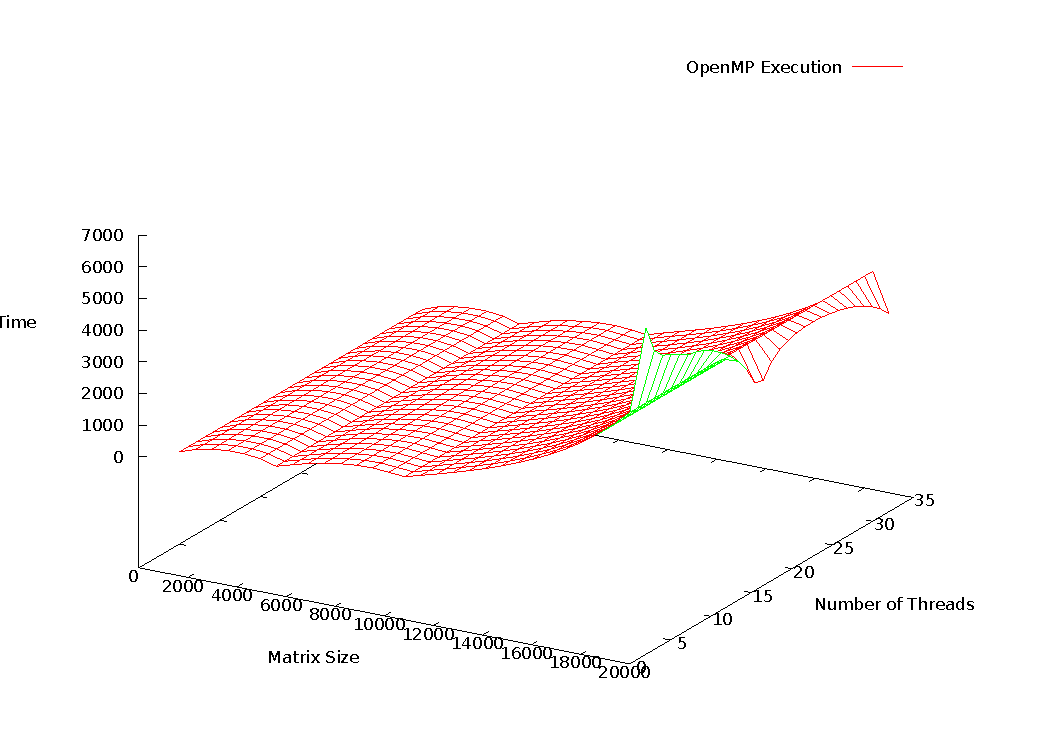
\includegraphics[height=3in,width=5in]{OpenMP/Plot.pdf}
\caption{OpenMP Decomposition Algorithm}
\end{center}
\end{figure}

\section{MPI Implementation}
\begin{itemize}
\item Cyclic distribution was used to accomplish LU factorization of the input square matrix.
\item Each node is responsible for computing its own block and broadcast the result to rest of the nodes.
\item Algorithm was evaluated for input matrix of sizes 1000, 5000, 10000 with a combination of 8, 16, 32 compute nodes working in parallel.
\item For a fixed number of compute nodes the algorithm showed uniform behavior.

\begin{figure}[H]
\begin{center}
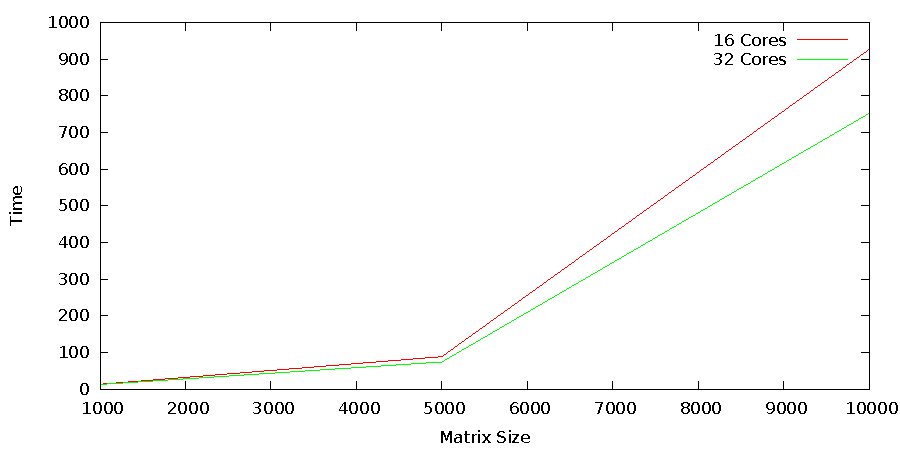
\includegraphics[height=3in,width=5in]{Graphs/mpi_siz_time.pdf}
\caption{MPI Performance for fixed number of compute nodes}
\end{center}
\end{figure}

\item For fixed workload the parallelism was more effective for larger workloads on maximum compute nodes.
\begin{figure}[H]
\begin{center}
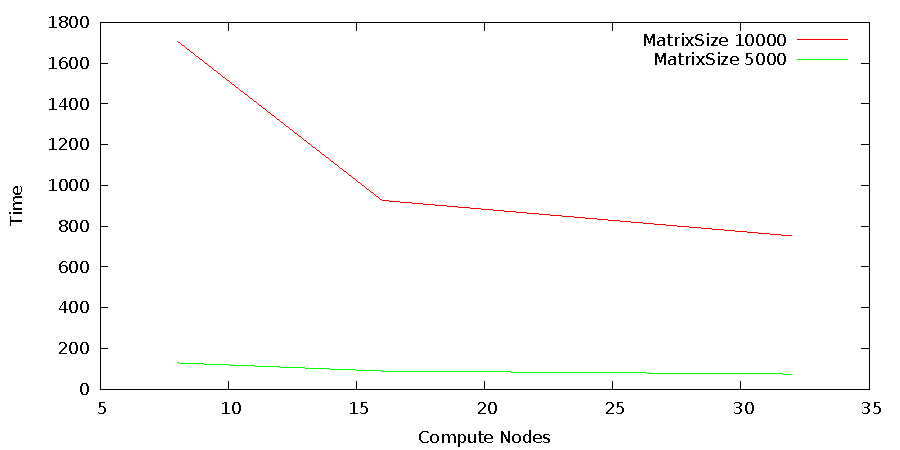
\includegraphics[height=3in,width=5in]{Graphs/mpi_core_time.pdf}
\caption{MPI Performance for fixed workload}
\end{center}
\end{figure}

\end{itemize}

\begin{figure}[H]
\begin{center}
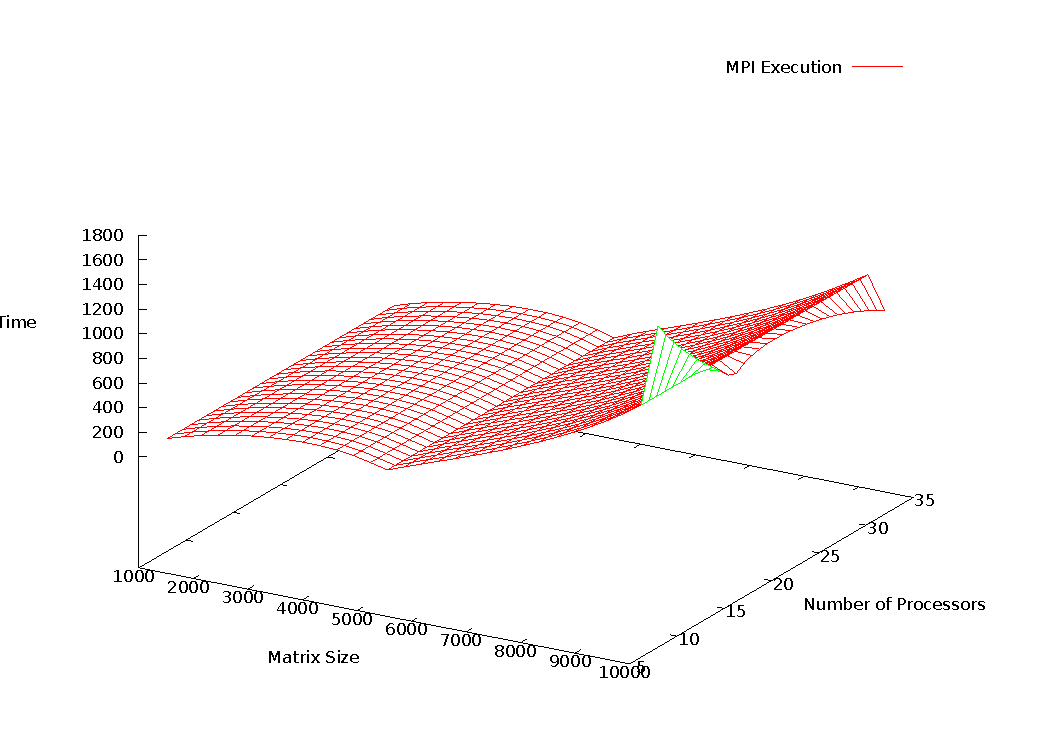
\includegraphics[height=3in,width=5in]{MPI/Plot.pdf}
\caption{MPI Decomposition Algorithm}
\end{center}
\end{figure}

\section{Comparison}
\begin{itemize}
\item Since, MPI involves communication overhead between different nodes, it was slower as compared to OpenMP. 

\begin{figure}[H]
\begin{center}
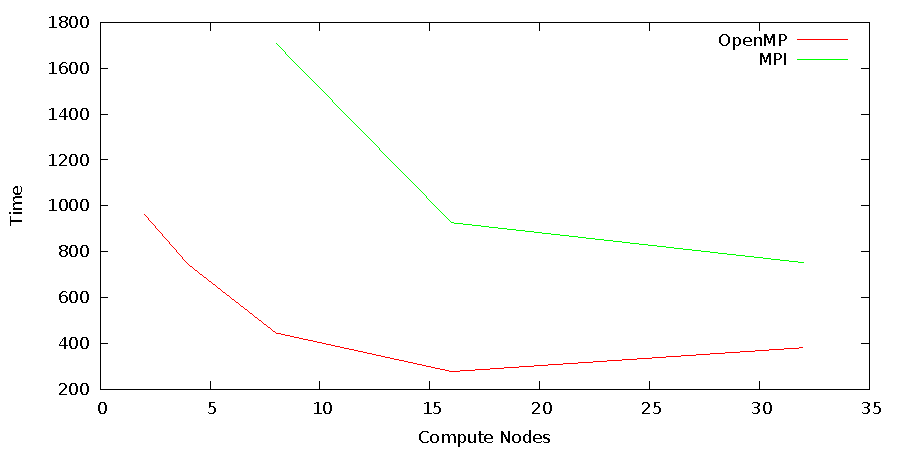
\includegraphics[height=3in,width=5in]{Graphs/omp_mpi_core_time.pdf}
\caption{OpenMP vs. MPI}
\end{center}
\end{figure}

\item As expected sequential algorithm turns out to be the worst performer of the three.

\begin{figure}[H]
\begin{center}
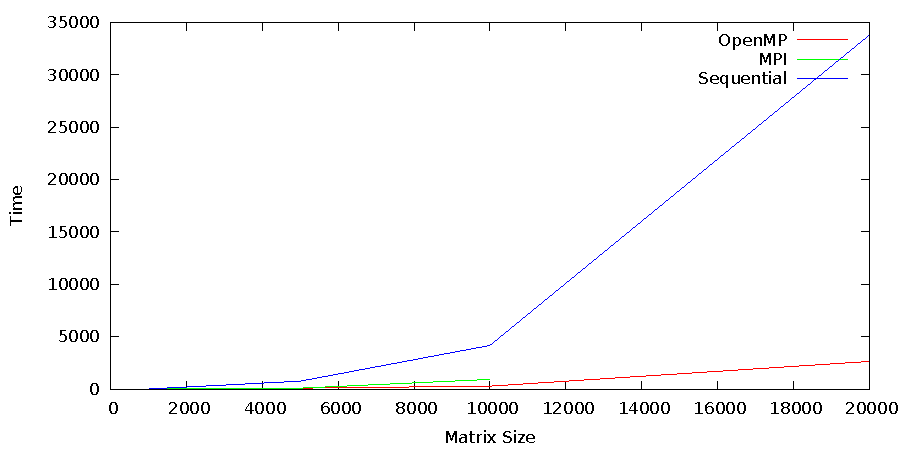
\includegraphics[height=3in,width=5in]{Graphs/omp_mpi_seq_siz_time.pdf}
\caption{Sequential vs. OpenMP vs. MPI}
\end{center}
\end{figure}

\end{itemize}

\section{Scalability}
LU factorization algorithm has a great extent of parallelization when scaled appropriately.
\end{document}